\section{Bayesian Statistics}

\subsection{Recommended References}
\begin{frame}{Bayesian Statistics - Recommended References}
	\begin{vfilleditems}
		\item \textcite{gelman2013bayesian} - Chapter 1: Probability and inference
		\item \textcite{mcelreath2020statistical} - Chapter 1: The Golem of Prague
		\item \textcite{gelman2020regression} - Chapter 3: Some basic methods in mathematics and probability
		\item \textcite{khanBayesianLearningRule2021}
		\item \textbf{Probability}:
		\begin{vfilleditems}
			\item A great textbook - \textcite{bertsekasIntroductionProbability2nd2008}
			\item Also a great textbook (skip the frequentist part)- \textcite{dekkingModernIntroductionProbability2010}
			\item Bayesian point-of-view and also a philosophical approach- \textcite{jaynesProbabilityTheoryLogic2003}
			\item Bayesian point-of-view with a simple and playful approach - \textcite{kurtBayesianStatisticsFun2019}
			\item Philosophical approach not so focused on mathematical rigor - \textcite{diaconisTenGreatIdeas2019}
		\end{vfilleditems}
	\end{vfilleditems}
\end{frame}

\subsection{What is Bayesian Statistics?}
\begin{frame}{What is Bayesian Statistics?}
	Bayesian statistics is a \textbf{data analysis approach based on Bayes' theorem}
	where available knowledge about the parameters of a statistical model
	is updated with the information of observed data.
	\parencite{gelman2013bayesian}.
	Previous knowledge is expressed as a \textbf{prior} distribution
	and combined with the observed data in the form of a \textbf{likelihood} function
	to generate a \textbf{posterior} distribution.
	The posterior can also be used to make predictions about future events.
\end{frame}

\subsubsection{What changes from Frequentist Statistics?}
\begin{frame}{What changes from Frequentist Statistics?}
	\begin{vfilleditems}
		\item \textbf{Flexibility} - probabilistic building blocks to
		construct a model\footnote{like LEGO}:
		\begin{vfilleditems}
			\item Probabilistic conjectures about parameters:
			\begin{vfilleditems}
				\item Prior
				\item Likelihood
			\end{vfilleditems}
		\end{vfilleditems}
		\item Better \textbf{uncertainty} treatment:
		\begin{vfilleditems}
			\item Coherence
			\item Propagation
			\item We don't use \textit{``if we sampled infinite times
				from a population that we do not observe...''}
		\end{vfilleditems}
		\item No \textbf{$p$-values}:
		\begin{vfilleditems}
			\item All statistical intuitions makes \textbf{sense}
			\item 95\% certainty that $\theta$'s parameter value is
			between $x$ and $y$
			\item Almost \textbf{impossible} to perform $p$-hacking
		\end{vfilleditems}
	\end{vfilleditems}
\end{frame}

\begin{frame}{A little bit more formal}
	\begin{vfilleditems}
		\item Bayesian Statistics uses probabilistic statements:
		\begin{vfilleditems}
			\item one or more parameters $\theta$
			\item unobserved data $\tilde{y}$
		\end{vfilleditems}
		\item These statements are conditioned on the observed values of $y$:
		\begin{vfilleditems}
			\item $P(\theta \mid y)$
			\item $P(\tilde{y} \mid y)$
		\end{vfilleditems}
		\item We also, implicitly, conditioned on the observed data from
		any covariate $x$
	\end{vfilleditems}
\end{frame}

\begin{frame}{Definition of Bayesian Statistics}
	\begin{defn}[Bayesian Statistics]
		The use of Bayes theorem as the procedure to \textbf{estimate
			parameters of interest $\theta$ or unobserved data $\tilde{y}$}.
		\parencite{gelman2013bayesian}
	\end{defn}
\end{frame}

\subsection{Probability}
\begin{frame}{PROBABILITY DOES NOT EXIST!\footnote{\textcite{definettiTheoryProbability1974}}}
	\begin{columns}
		\begin{column}{0.8\textwidth}
			\begin{vfilleditems}
				\item Yes, probability does not exist ...
				\item Or even better, probability as a physical quantity,
				objective chance, \textbf{does NOT exist}
				\item if we disregard objetive chance \textit{nothing is lost}
				\item The math of inductive rationality remains
				\textbf{exactly the same}
			\end{vfilleditems}
		\end{column}
		\begin{column}{0.2\textwidth}
			\centering
			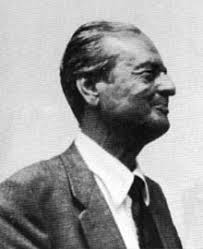
\includegraphics[width=0.9\columnwidth]{finetti.jpg}
		\end{column}
	\end{columns}
\end{frame}

\begin{frame}{PROBABILITY DOES NOT EXIST!\footnote{\textcite{definettiTheoryProbability1974}}}
	\begin{columns}
		\begin{column}{0.6\textwidth}
			\begin{vfilleditems}
				\small
				\item Consider flipping a biased coin
				\item The trials are considered independent and, as a result,
				have an important property: \textbf{the order does not matter}
				\item The frequency is considered a \textbf{sufficient statistic}
				\item Saying that order does not matter or saying that the only thing that
				matters is frequency are two ways of saying the same thing
				\item We say that the probability is \textbf{invariant under permutations}
			\end{vfilleditems}
		\end{column}
		\begin{column}{0.4\textwidth}
			\begin{tikzpicture}[
					scale=0.55,
					transform shape, thick,
					every node/.style = {draw, circle, minimum size = 10mm},
					grow = down,  % alignment of characters
					level 1/.style = {sibling distance=3cm},
					level 2/.style = {sibling distance=1.5cm},
					level 3/.style = {sibling distance=3cm},
					level distance = 3cm,
					head/.style = {fill = orange!90!blue,
							label = center:\textsf{\Large H}},
					tail/.style = {fill = blue!70!yellow, text = black,
							label = center:\textsf{\Large T}}
				]
				\node[shape = circle split, draw, line width = 1pt,
					minimum size = 10mm, inner sep = 0mm, font = \sffamily\large,
					rotate=30] (Start)
				{ \rotatebox{-30}{H} \nodepart{lower} \rotatebox{-30}{T}}
				child {   node [head] (A) {}
						child { node [head] (B) {}}
						child { node [tail] (C) {}}
					}
				child {   node [tail] (D) {}
						child { node [head] (E) {}}
						child { node [tail] (F) {}}
					};

				% Filling the root (Start)
				\begin{scope}[on background layer, rotate=30]
					\fill[head] (Start.base) ([xshift = 0mm]Start.east) arc (0:180:5mm)
					-- cycle;
					\fill[tail] (Start.base) ([xshift = 0pt]Start.west) arc (180:360:5mm)
					-- cycle;
				\end{scope}

				% Labels
				\begin{scope}[nodes = {draw = none}]
					\path (Start) -- (A) node [near start, left]  {$0.5$};
					\path (A)     -- (B) node [near start, left]  {$0.5$};
					\path (A)     -- (C) node [near start, right] {$0.5$};
					\path (Start) -- (D) node [near start, right] {$0.5$};
					\path (D)     -- (E) node [near start, left]  {$0.5$};
					\path (D)     -- (F) node [near start, right] {$0.5$};
					\begin{scope}[nodes = {below = 11pt}]
						\node at (B) {$0.25$};
						\node at (C) {$0.25$};
						\node at (E) {$0.25$};
						\node at (F) {$0.25$};
					\end{scope}
				\end{scope}
			\end{tikzpicture}
		\end{column}
	\end{columns}
\end{frame}

\begin{frame}{Probability Interpretations}
	\begin{vfilleditems}
		\item \textbf{Objective} - frequency in the long run for an event:
		\begin{vfilleditems}
			\item $P(\text{rain}) = \frac{\text{days that rained}}{\text{total days}}$
			\item $P(\text{me being elected president}) = 0$ (never occurred)
		\end{vfilleditems}
		\item \textbf{Subjective} - degrees of belief in an event:
		\begin{vfilleditems}
			\item $P(\text{rain}) = \text{degree of belief that will rain}$
			\item $P(\text{me being elected president}) = 10^{-10}$ (highly unlikely)
		\end{vfilleditems}
	\end{vfilleditems}
\end{frame}

\subsubsection{What is Probability?}
\begin{frame}{What is Probability?}
	\begin{defn}[Probability]
		We define $A$ is an event and $P(A)$ the probability of event $A$.
		$P(A)$ has to be between $0$ and $1$, where higher values defines
		higher probability of $A$ happening.
		$$\begin{aligned}
				P(A)   & \in \mathbb{R} \\
				P(A)   & \in [0,1]      \\
				0 \leq & P(A) \leq 1
			\end{aligned}$$
	\end{defn}
\end{frame}

\begin{frame}{Probability Axioms\footnote{\textcite{kolmogorovFoundationsTheoryProbability1933}}}
	\begin{columns}
		\begin{column}{0.8\textwidth}
			\begin{vfilleditems}
				\item \textbf{Non-negativity}: For every $A$:
				$$P(A) \geq 0$$
				\item \textbf{Additivity}: For every two \textit{mutually exclusive}
				$A$ and $B$:
				$$P(A) = 1 - P(B) \text{ and } P(B) = 1 - P(A)$$
				\item \textbf{Normalization}: The probability of all possible
				events $A_1, A_2, \dots$ must sum up to $1$:
				$$\sum_{n \in \mathbb{N}} A_n = 1$$
			\end{vfilleditems}
		\end{column}
		\begin{column}{0.2\textwidth}
			\centering
			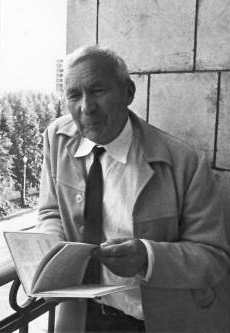
\includegraphics[width=0.9\columnwidth]{kolmogorov.jpg}
		\end{column}
	\end{columns}
\end{frame}

\begin{frame}{Sample Space}
	\begin{vfilleditems}
		\item Discrete $$\Theta = \left\{1, 2, \ldots \right\}$$
		\item Continuous $$\Theta \in \left(-\infty, \infty \right)$$
	\end{vfilleditems}
\end{frame}

\begin{frame}{Discrete Sample Space}
	8 planets in our solar system:
	\begin{vfilleditems}
		\item Mercury - $\mercury$
		\item Venus - $\venus$
		\item Earth - $\earth$
		\item Mars $\mars$
		\item Jupiter - $\jupiter$
		\item Saturn $\saturn$
		\item Uranus - $\uranus$
		\item Neptune $\neptune$
	\end{vfilleditems}
\end{frame}

\begin{frame}[fragile]{Discrete Sample Space\footnote{figure adapted from \href{https://github.com/betanalpha/stan_intro}{Michael Betancourt (CC-BY-SA-4.0)}}}
	\footnotesize
	\begin{figure}
		\centering
		\subfigure{
			\begin{tikzpicture}[scale=0.25, thick]
				\draw[color=black] (-25, 0) to (10, 0);
				\node[] at (-15, 0) {The planet has a magnetic field};
				\node[] at (7, 2) {$\theta \in E_{1}$};

				\fill[color=gray60] (0, 0) circle (25pt) node[color=black] {$\mercury$};
				\fill[color=blue] (2, 0) circle (25pt) node[color=black] {$\venus$};
				\fill[color=blue] (4, 0) circle (25pt) node[color=black] {$\earth$};
				\fill[color=gray60] (6, 0) circle (25pt) node[color=black] {$\mars$};
				\fill[color=blue] (8, 0) circle (25pt) node[color=black] {$\jupiter$};
				\fill[color=blue] (10, 0) circle (25pt) node[color=black] {$\saturn$};
				\fill[color=blue] (12, 0) circle (25pt) node[color=black] {$\uranus$};
				\fill[color=blue] (14, 0) circle (25pt) node[color=black] {$\neptune$};
			\end{tikzpicture}
		}
		%
		\subfigure{
			\begin{tikzpicture}[scale=0.25, thick]
				\draw[color=black] (-25, 0) to (10, 0);
				\node[] at (-15, 0) {The planet has moon(s)};
				\node[] at (7, 2) {$\theta \in E_{2}$};

				\fill[color=gray60] (0, 0) circle (25pt) node[color=black] {$\mercury$};
				\fill[color=gray60] (2, 0) circle (25pt) node[color=black] {$\venus$};
				\fill[color=blue] (4, 0) circle (25pt) node[color=black] {$\earth$};
				\fill[color=blue] (6, 0) circle (25pt) node[color=black] {$\mars$};
				\fill[color=blue] (8, 0) circle (25pt) node[color=black] {$\jupiter$};
				\fill[color=blue] (10, 0) circle (25pt) node[color=black] {$\saturn$};
				\fill[color=blue] (12, 0) circle (25pt) node[color=black] {$\uranus$};
				\fill[color=blue] (14, 0) circle (25pt) node[color=black] {$\neptune$};
			\end{tikzpicture}
		}
		%
		\subfigure{
			\begin{tikzpicture}[scale=0.25, thick]
				\draw[color=black] (-25, 0) to (10, 0);
				\node[] at (-15, 0) {The planet has a magnetic field \textit{and} moon(s)};
				\node[] at (7, 2) {$\theta \in E_{1} \cap E_{2}$};

				\fill[color=gray60] (0, 0) circle (25pt) node[color=black] {$\mercury$};
				\fill[color=gray60] (2, 0) circle (25pt) node[color=black] {$\venus$};
				\fill[color=blue] (4, 0) circle (25pt) node[color=black] {$\earth$};
				\fill[color=gray60] (6, 0) circle (25pt) node[color=black] {$\mars$};
				\fill[color=blue] (8, 0) circle (25pt) node[color=black] {$\jupiter$};
				\fill[color=blue] (10, 0) circle (25pt) node[color=black] {$\saturn$};
				\fill[color=blue] (12, 0) circle (25pt) node[color=black] {$\uranus$};
				\fill[color=blue] (14, 0) circle (25pt) node[color=black] {$\neptune$};
			\end{tikzpicture}
		}
		%
		\subfigure{
			\begin{tikzpicture}[scale=0.25, thick]
				\node[] at (-15, 0) {The planet has a magnetic field \textit{or} moon(s)};
				\node[] at (7, 2) {$\theta \in E_{1} \cup E_{2}$};

				\fill[color=gray60] (0, 0) circle (25pt) node[color=black] {$\mercury$};
				\fill[color=blue] (2, 0) circle (25pt) node[color=black] {$\venus$};
				\fill[color=blue] (4, 0) circle (25pt) node[color=black] {$\earth$};
				\fill[color=blue] (6, 0) circle (25pt) node[color=black] {$\mars$};
				\fill[color=blue] (8, 0) circle (25pt) node[color=black] {$\jupiter$};
				\fill[color=blue] (10, 0) circle (25pt) node[color=black] {$\saturn$};
				\fill[color=blue] (12, 0) circle (25pt) node[color=black] {$\uranus$};
				\fill[color=blue] (14, 0) circle (25pt) node[color=black] {$\neptune$};
			\end{tikzpicture}
		}
		%
		\subfigure{
			\begin{tikzpicture}[scale=0.25, thick]
				\node[] at (-15, 0) {The planet does \textit{not} have a magnetic field};
				\node[] at (7, 2) {$\theta \in \neg E_{1}$};

				\fill[color=blue] (0, 0) circle (25pt) node[color=black] {$\mercury$};
				\fill[color=gray60] (2, 0) circle (25pt) node[color=black] {$\venus$};
				\fill[color=gray60] (4, 0) circle (25pt) node[color=black] {$\earth$};
				\fill[color=blue] (6, 0) circle (25pt) node[color=black] {$\mars$};
				\fill[color=gray60] (8, 0) circle (25pt) node[color=black] {$\jupiter$};
				\fill[color=gray60] (10, 0) circle (25pt) node[color=black] {$\saturn$};
				\fill[color=gray60] (12, 0) circle (25pt) node[color=black] {$\uranus$};
				\fill[color=gray60] (14, 0) circle (25pt) node[color=black] {$\neptune$};
			\end{tikzpicture}
		}
		%
	\end{figure}
\end{frame}

\begin{frame}{Continuous Sample Space\footnote{
			figure adapted from \href{https://github.com/betanalpha/stan_intro}{Michael Betancourt (CC-BY-SA-4.0)}}
	}
	\footnotesize
	\begin{figure}
		\centering
		\subfigure{
			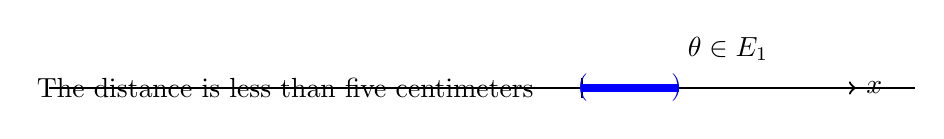
\begin{tikzpicture}[scale=0.25, thick]
				\draw[color=black] (-27, 0) to (17, 0);
				\node[align=center] at (-15, 0) {The distance is less than five centimeters};
				\node[] at (7.5, 2) {$\theta \in E_{1}$};

				\draw[|->] (0, 0) -- (14,0) node[right] {$x$};
				\draw[line width=1mm, color=blue] (0, 0) node[] {$\,($} -- (5, 0) node[] {$\!)$};
			\end{tikzpicture}
		}
		%
		\subfigure{
			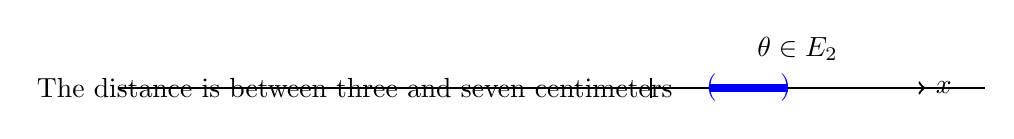
\begin{tikzpicture}[scale=0.25, thick]
				\draw[color=black] (-27, 0) to (17, 0);
				\node[align=center] at (-15, 0) {The distance is between three and seven centimeters};
				\node[] at (7.5, 2) {$\theta \in E_{2}$};

				\draw[|->] (0, 0) -- (14,0) node[right] {$x$};
				\draw[line width=1mm, color=blue] (3, 0) node[] {$\,($} -- (7,0) node[] {$\!)$};

			\end{tikzpicture}
		}
		%
		\subfigure{
			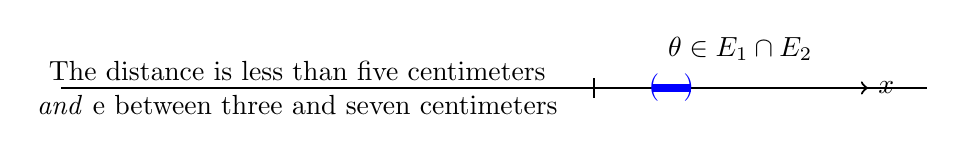
\begin{tikzpicture}[scale=0.25, thick]
				\draw[color=black] (-27, 0) to (17, 0);
				\node[align=center] at (-15, 0) {The distance is less than five centimeters \\ \textit{and} e between three and seven centimeters};
				\node[] at (7.5, 2) {$\theta \in E_{1} \cap E_{2}$};

				\draw[|->] (0, 0) -- (14,0) node[right] {$x$};
				\draw[line width=1mm, color=blue] (3, 0) node[] {$\,($} -- (5, 0) node[] {$\!)$};
			\end{tikzpicture}
		}
		%
		\subfigure{
			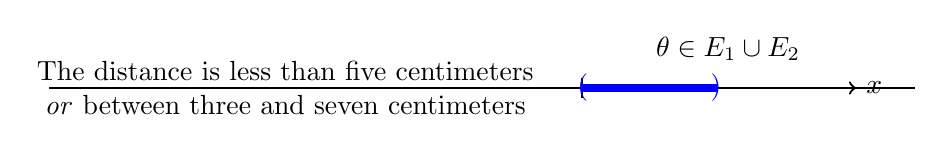
\begin{tikzpicture}[scale=0.25, thick]
				\draw[color=black] (-27, 0) to (17, 0);
				\node[align=center] at (-15, 0) {The distance is less than five centimeters \\ \textit{or} between three and seven centimeters};
				\node[] at (7.5, 2) {$\theta \in E_{1} \cup E_{2}$};

				\draw[|->] (0, 0) -- (14, 0) node[right] {$x$};
				\draw[line width=1mm, color=blue] (0, 0) node[] {$\,($} -- (7, 0) node[] {$\!)$};
			\end{tikzpicture}
		}
		%		%
		\subfigure{
			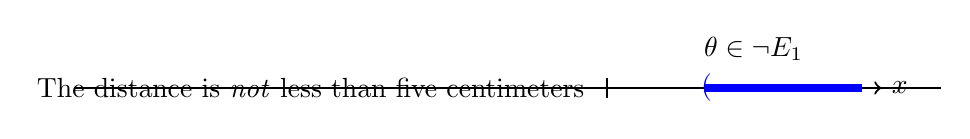
\begin{tikzpicture}[scale=0.25, thick]
				\draw[color=black] (-27, 0) to (17, 0);
				\node[align=center] at (-15, 0) {The distance is \textit{not} less than five centimeters};
				\node[] at (7.5, 2) {$\theta \in \neg E_{1}$};

				\draw[|->] (0, 0) -- (14, 0) node[right] {$x$};
				\draw[line width=1mm, color=blue] (5, 0) node[] {$\,($} -- (13, 0);
			\end{tikzpicture}
		}
	\end{figure}
\end{frame}

\begin{frame}{Discrete versus Continuous Parameters}

	Everything that has been exposed here was under the assumption that the
	parameters are discrete.
	This was done with the intent to provide an intuition what is probability.
	Not always we work with discrete parameters.
	Parameters can be continuous, such as: age, height, weight etc.
	But don't despair!
	All probability rules and axioms are valid also for continuous parameters.
	The only thing we have to do is to change all sum $\sum$ for integrals $\int$.
	For example, the third axiom of \textbf{Normalization} for \textit{continuous}
	random variables becomes:
	$$
		\int_{x \in X} p(x) dx = 1.
	$$
\end{frame}


\begin{frame}{Conditional Probability}
	\begin{defn}[Conditional Probability]
		Probability of an event occurring in case another has occurred or not. \newline \newline
		The notation we use is $P( A \mid B )$, that read as ``the probability of
		observing $A$ given that we already observed $B$''. \newline \newline
		$$
			\begin{aligned}
				P(A \mid B) & = \frac{\text{number of elements in$A$ e $B$}}{\text{number of elements in $B$}} \\
				P(A \mid B) & = \frac{P(A \cap B)}{(B)}
			\end{aligned}
		$$
		\newline \hspace{0.7\textwidth}
		{\footnotesize assuming that $P(B) > 0$}.
	\end{defn}
\end{frame}

\begin{frame}{Example of Conditional Probability}
	\begin{example}[Poker Texas Hold'em]
		\begin{vfilleditems}
			\item \textbf{Sample Space}: $52$ cards in a deck, $13$ types of cards and $4$ types of suits.
			\item $P(A)$: Probability of being dealt an Ace $\left( \frac{4}{52} = \frac{1}{13}\right)$
			\item $P(K)$: Probability of being dealt a King $\left( \frac{4}{52} = \frac{1}{13} \right)$
			\item $P(A \mid K)$: Probability of being dealt an Ace, given that you have already a King $\left( \frac{4}{51} \approx 0.078 \right)$
			\item $P(K \mid A)$: Probability of being dealt a King, given that you have already an Ace $\left( \frac{4}{51} \approx 0.078 \right)$
		\end{vfilleditems}
	\end{example}
\end{frame}

\begin{frame}{Caution! Not always $P(A \mid B) = P(B \mid A)$}
	In the previous example we have the symmetry $P(A \mid K) = P(K \mid A)$,
	\textbf{but not always this is true}\footnote{
		More specific, if the basal rates $P(A)$ and $P(B)$ aren't equal,
		the symmetry is broken $P(A \mid B) \neq P(B \mid A)$}
	\begin{example}[The Pope is catholic]
		\begin{vfilleditems}
			\small{
				\item $P(\text{pope})$:
				Probability of some random person being the Pope,
				something really small, 1 in 8 billion $\left( \frac{1}{8 \cdot 10^9} \right)$
				\item $P(\text{catholic})$:
				Probability of some random person being catholic,
				1.34 billion in 8 billion $\left( \frac{1.34}{8} \approx 0.17 \right)$
				\item $P(\text{catholic} \mid \text{pope})$:
				Probability of the Pope being catholic $\left( \frac{999}{1000} = 0.999 \right)$
				\item $P(\text{pope} \mid \text{catholic})$:
				Probability of a catholic person being the Pope $\left( \frac{1}{1.34 \cdot 10^9} \cdot 0.999 \approx 7.46 \cdot 10^{-10} \right)$
			}
			\item \large{\textbf{Hence}: $P(\text{catholic} \mid \text{pope}) \neq P(\text{pope} \mid \text{catholic})$}
		\end{vfilleditems}
	\end{example}
\end{frame}

\begin{frame}{A Probability Textbook Classic}
	\begin{columns}
		\begin{column}{0.6\textwidth}
			\begin{example}[Monty Hall]
				\begin{vfilleditems}
					\small
					\item A TV presenter shows you 3 doors
					\item One of them has a prize: a car!
					The others have a goat
					\item You must choose a door (that is not open or revealed)
					\item In this moment, the presenter opens one of the other two doors
					that you did not choose,
					revealing one of the two goats
					\item The presenter then asks you
					``Do you want to change your door or stay with your choice?''
				\end{vfilleditems}
			\end{example}
		\end{column}
		\begin{column}{0.4\textwidth}
			\begin{figure}
				\centering
				\def\svgwidth{\columnwidth}
				\input{../images/monty_hall.pdf_tex}
			\end{figure}
		\end{column}
	\end{columns}
\end{frame}

\begin{frame}{Solution for the Monty Hall Problem}
	\begin{idea}[Probability of winning a car]
		$$
			\begin{aligned}
				P(\text{car} \mid C_i) & = \frac{1}{3}                                                                                                                    \\
				P(\text{car})          & = \frac{1}{3} \cdot P(\text{car} \mid C_1) + \frac{1}{3} \cdot P(\text{car} \mid C_2) + \frac{1}{3} \cdot P(\text{car} \mid C_3) \\
				P(\text{car})          & = \frac{\sum^3_{i=1}P(\text{car} \mid C_i)}{3}                                                                                   \\
				P(\text{car})          & = \frac{1}{3}
			\end{aligned}
		$$
	\end{idea}
	\vfill \vfill
	$C_i$ is the event that the car is behind door $i$, $i=1,2,3$
\end{frame}

\begin{frame}[t]{Solution for the Monty Hall Problem}
	\begin{columns}[t]
		\begin{column}{0.5\textwidth}
			{\Large \textbf{Scenario 1}: Don't change doors} \newline \newline
			Simple: $$\frac{1}{3}$$
		\end{column}
		\begin{column}{0.5\textwidth}
			{\Large \textbf{Scenario 2}: Change doors} \newline \newline
			Choose any door $i$ to be $C_i = 0$
			\vfill
			$$
				\begin{aligned}
					P(\text{car}) & = 0 \cdot P(\text{car} \mid C_i) + \frac{1}{3} + \frac{1}{3} \\
					P(\text{car}) & = \frac{2}{3}
				\end{aligned}
			$$
		\end{column}
	\end{columns}
\end{frame}

\begin{frame}{Visualization of the Monty Hall Problem}
	\begin{figure}
		\centering
		\subfigure{
			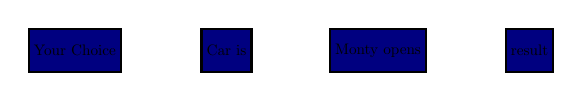
\begin{tikzpicture}[
					scale=0.55,
					header/.style = {draw, rectangle, fill = blue!50!black, minimum size = 10mm},
					level distance = 3.5cm,
					transform shape, thick,
					grow = right, sloped,
				]
				\node[header] {Your Choice}
				child{
						node[header] {Car is}
						edge from parent[draw=none]
						child{
								node[header] {Monty opens}
								edge from parent[draw=none]
								child{
										node[header] {result}
										edge from parent[draw=none]
									}
							}
					};
			\end{tikzpicture}
		}
		%
		\subfigure{
			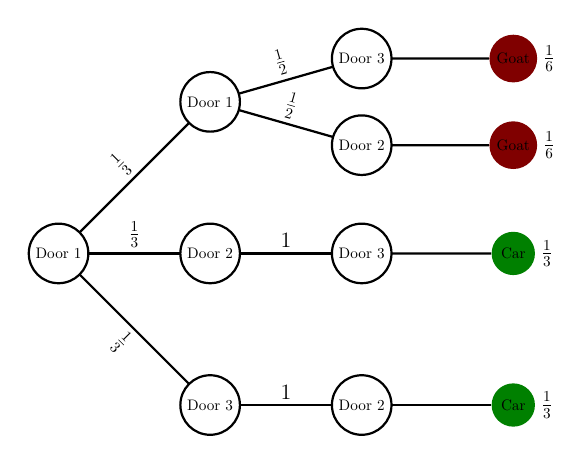
\begin{tikzpicture}[
					scale=0.55,
					door/.style = {draw, circle, minimum size = 10mm},
					car/.style = {circle, fill = green!50!black, minimum size = 10mm},
					goat/.style = {circle, fill = red!50!black, minimum size = 10mm},
					level distance = 3.5cm,
					transform shape, thick,
					grow = right, sloped,
					level 1/.style = {sibling distance=3.5cm},
					level 2/.style = {sibling distance=2cm},
					level 3/.style = {sibling distance=3cm}
				]
				\node[door] {Door 1}
				child {
				node[door] {Door 3}
				child {
				node[door] {Door 2}
				child {
				node[car, label=right:{\Large$\frac{1}{3}$}] {Car}
				}
				edge from parent
				node[above] {\Large$1$}
				}
				edge from parent
				node[below] {\Large$\frac{1}{3}$}
				}
				child {
				node[door] {Door 2}
				child {
				node[door] {Door 3}
				child {
				node[car, label=right:{\Large$\frac{1}{3}$}] {Car}
				}
				edge from parent
				node[above] {\Large$1$}
				}
				edge from parent
				node[above] {\Large$\frac{1}{3}$}
				}
				child {
				node[door] {Door 1}
				child {
				node[door] {Door 2}
				child {
				node[goat, label=right:{\Large$\frac{1}{6}$}] {Goat}
				}
				edge from parent
				node[above]  {\Large$\frac{1}{2}$}
				}
				child {
				node[door] {Door 3}
				child {
				node[goat, label=right:{\Large$\frac{1}{6}$}] {Goat}
				}
				edge from parent
				node[above]  {\Large$\frac{1}{2}$}
				}
				edge from parent
				node[above] {\Large$\frac{1}{3}$}
				};
			\end{tikzpicture}
		}
	\end{figure}
\end{frame}

\begin{frame}{Joint Probability}
	\begin{defn}[Joint Probability]
		Probability of two or more events occurring. \newline \newline
		The notation we use is $P(A, B)$, that read as
		``the probability of observing $A$ and also observing $B$''. \newline \newline
		$$
			\begin{aligned}
				P(A,B) & = \text{number of elements in $A$ or $B$} \\
				P(A,B) & = P(A \cup B)                             \\
				P(A,B) & = P(B,A)
			\end{aligned}
		$$
	\end{defn}
\end{frame}

\begin{frame}{Example of Joint Probability}
	\begin{example}[Revisiting Poker Texas Hold'em]
		\begin{vfilleditems}
			{\footnotesize
				\item \textbf{Sample Space}: $52$ cards in a deck, $13$ types of cards and $4$ types of suits.
				\item $P(A)$: Probability of being dealt an Ace $\left( \frac{4}{52} = \frac{1}{13}\right)$
				\item $P(K)$: Probability of being dealt a King $\left( \frac{4}{52} = \frac{1}{13} \right)$
				\item $P(A \mid K)$: Probability of being dealt an Ace, given that you have already a King $\left( \frac{4}{51} \approx 0.078 \right)$
				\item $P(K \mid A)$: Probability of being dealt a King, given that you have already an Ace $\left( \frac{4}{51} \approx 0.078 \right)$
			}
			\item $P(A, K)$: Probability of being dealt an Ace \textit{and} being dealt a King
			$$
				\begin{aligned}
					P(A, K)                         & = P(K, A)                         \\
					P(A) \cdot P(K \mid A)          & = P(K) \cdot P(A \mid K)          \\
					\frac{1}{13} \cdot \frac{4}{51} & = \frac{1}{13} \cdot \frac{4}{51} \\
					                                & \approx 0.006
				\end{aligned}
			$$
		\end{vfilleditems}
	\end{example}
\end{frame}

%% Bivariate Normal adapted from: https://github.com/walmes/Tikz/blob/master/src/bivariate-normal.pgf
\begin{frame}{Visualization of Joint Probability versus Conditional Probability}
	\centering
	\begin{tikzpicture}[scale=0.9]
		\begin{axis}[
				domain   = -3.5:3.5,
				domain y = -3.5:3.5,
				view = {-70}{20},
				title={$P(X,Y)$ versus $P(X \mid Y=-0.75)$},
				xlabel={$X$},
				ylabel={$Y$},
				% zlabel={$SSE(\beta_0, \beta_1)$},
				zmin = -0,
				%xticklabels=\empty,
				%yticklabels=\empty,
				zticklabels=\empty,
				xtick=\empty,
				ytick={-0.75},
				ztick=\empty,
				axis z line*=none,
				axis y line*=left,
				axis x line*= bottom]
			\addplot3 [
				domain = -3.5:3.5,
				samples = 50, samples y = 0,
				thick, smooth, color = red, fill = orange, opacity = 0.75]
			(x, -0.75, {conditionalbinormal(-0.75, 0, 1, 0, 1, 0.75)});

			\draw (-3.5, -0.75, 0) -- (3.5, -0.75, 0);

			\addplot3 [
				surf,
				domain = -3.5:3.5,
				samples = 50,
				opacity = 0.15,
				faceted color = colorB,
				colormap = {blueblack}{
						color = (colorB)
						color = (colorA!50!white)
						color = (colorA)}]
			{binormal(0, 1, 0, 1, 0.7)};
		\end{axis}
	\end{tikzpicture}
\end{frame}

%% Contour plot adapted from: https://tex.stackexchange.com/a/31713/200209
\begin{frame}{Visualization of Joint Probability versus Conditional Probability}
	\begin{columns}
		\begin{column}{0.5\textwidth}
			\centering
			\begin{tikzpicture}[scale=0.5]
				\begin{axis}[
						view={0}{90},
						axis equal,
						enlarge y limits=true,
						title={$P(X,Y)$},
						xlabel={$X$},
						ylabel={$Y$},
						xtick=\empty,
						ytick={-0.75}
					]

					\draw[red, line width=2pt] (-3.5, -0.75) -- (3.5, -0.75);

					\addplot3[contour gnuplot={labels=false},domain=-3.5:3.5,domain y=-3.5:3.5]
					{exp(-( x^2 + y^2)/3 )};

				\end{axis}
			\end{tikzpicture}
		\end{column}
		\begin{column}{0.5\textwidth}
			\centering
			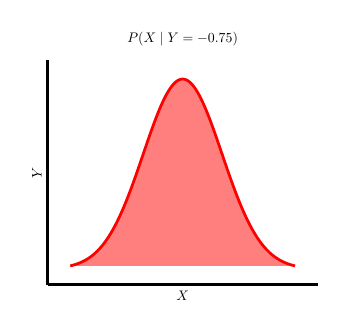
\begin{tikzpicture}[scale=0.5]
				\begin{axis}[every axis plot, line width=2pt,
						title={$P(X \mid Y=-0.75)$},
						xlabel={$X$},
						ylabel={$Y$},
						xtick=\empty,
						ytick=\empty,
						domain=-3.5:3.5,samples=200,
						axis x line*=bottom,  % no box around the plot, only x and y axis
						axis y line*=left,    % the * suppresses the arrow tips
						enlarge x limits=true % extend the axes a bit
					]

					\addplot [red, fill = red, fill opacity = 0.5] {exp(-( x^2 + -0.75^2)/3 )};
				\end{axis}
			\end{tikzpicture}
		\end{column}
	\end{columns}
\end{frame}

\subsubsection{Bayes Theorem}
\begin{frame}{Who was Thomas Bayes?}
	\begin{columns}
		\begin{column}{0.8\textwidth}
			\begin{vfilleditems}
				\item \small \textbf{Thomas Bayes} (1701 - 1761) was a statistician, philosopher
				and Presbyterian minister who is known for formulating a specific
				case of the theorem that bears his name: Bayes' theorem.
				\item \small Bayes never published what would become his most famous
				accomplishment; his notes were edited and published posthumously by
				his friend \textbf{Richard Price}.
				\item \small The theorem official name is \textbf{Bayes-Price-Laplace},
				because \textbf{Bayes} was the first to discover,
				\textbf{Price} got his notes, transcribed into mathematical notation,
				and read to the Royal Society of London,
				and \textbf{Laplace} independently rediscovered the theorem without
				having previous contact in the end of the XVIII century in France
				while using probability for statistical inference with census
				data in the Napoleonic era.
			\end{vfilleditems}
		\end{column}
		\begin{column}{0.2\textwidth}
			\centering
			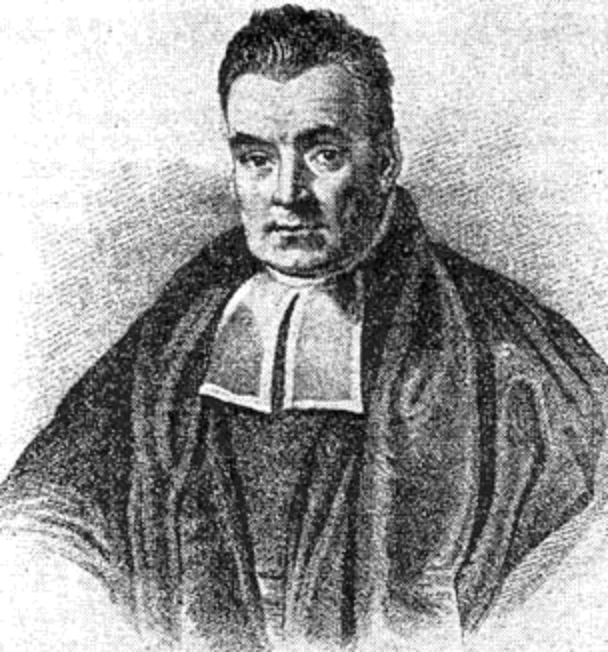
\includegraphics[width=0.9\columnwidth]{thomas_bayes.png}
		\end{column}
	\end{columns}
\end{frame}

\begin{frame}{Bayes Theorem}
	\begin{theorem}[Bayes]
		Tells us how to ``invert'' conditional probability: \newline \newline
		$$P(A \mid B) = \frac{P(A) \cdot P(B \mid A)}{P(B)}$$
	\end{theorem}
\end{frame}

\begin{frame}{Bayes' Theorem Proof}
	Remember the following probability identity:
	$$
		\begin{aligned}
			P(A,B)                 & = P(B,A)                 \\
			P(A) \cdot P(B \mid A) & = P(B) \cdot P(A \mid B)
		\end{aligned}
	$$

	OK, now divide everything by $P(B)$:
	$$
		\begin{aligned}
			\frac{P(A) \cdot P(B \mid A)}{P(B)} & = \frac{P(B) \cdot \quad P(A \mid B)}{P(B)} \\
			                                    &                                             \\
			\frac{P(A) \cdot P(B \mid A)}{P(B)} & = P(A \mid B)                               \\
			P(A \mid B)                         & = \frac{P(A) \cdot P(B \mid A)}{P(B)}
		\end{aligned}
	$$
\end{frame}

\begin{frame}{Another Probability Textbook Classic\footnote{Adapted from: \href{https://www.yudkowsky.net/rational/bayes}{Yudkowski - \textit{An Intuitive Explanation of Bayes’ Theorem}}.}}
	\begin{example}[Breast Cancer]
		\small
		How accurate is a \textbf{breast cancer} test?
		\begin{vfilleditems}
			\item \footnotesize 1\% of women have \textbf{breast cancer} (Prevalence)
			\item \footnotesize 80\% of mammograms detect \textbf{breast cancer} (True Positive)
			\item \footnotesize 9.6\% of mammograms detect \textbf{breast cancer} when there is no incidence (False Positive)
		\end{vfilleditems}
		$$
			\begin{aligned}
				P(C \mid +) & = \frac{P(+ \mid C) \cdot P(C)}{P(+)}                                                      \\
				P(C \mid +) & = \frac{P(+ \mid C) \cdot P(C)}{P(+ \mid C) \cdot P(C) + P(+ \mid \neg C) \cdot P(\neg C)} \\
				P(C \mid +) & = \frac{0.8 \cdot 0.01}{0.8 \cdot 0.01 + 0.096 \cdot 0.99}                                 \\
				P(C \mid +) & \approx 0.0776
			\end{aligned}
		$$
	\end{example}
\end{frame}


\begin{frame}{Why Bayes' Theorem is Important?}
	\begin{idea}[We can Invert the Conditional Probability]
		$$
			\begin{aligned}
				P(\text{hypothesis} \mid \text{data}) = \frac{P(\text{data} \mid \text{hypothesis}) \cdot P(\text{hypothesis})}{P(\text{data})}
			\end{aligned}
		$$
	\end{idea}
	But isn't this the $p$-value? \textcolor{red}{\textbf{NO!}}
\end{frame}

\subsection{Frequentist versus Bayesian}
\subsubsection{What are $p$-values and Confidence Intervals}
\begin{frame}{What are $p$-values?}
	\begin{defn}[$p$-value]
		$p$-value is the probability of obtaining results at least as
		extreme as the observed,
		given that the null hypothesis $H_0$ is true:
		$$P(D \mid H_0)$$
	\end{defn}
\end{frame}

\begin{frame}{What $p$-value is \textbf{not}!}
	\centering
	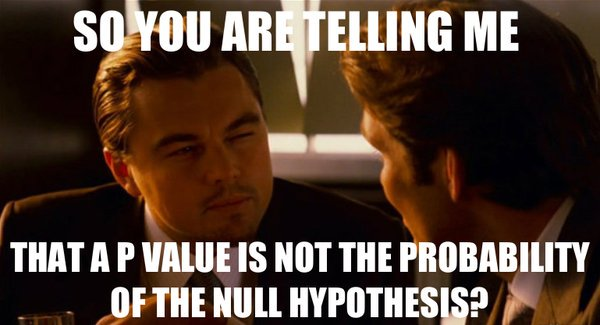
\includegraphics[width=0.7\textwidth]{meme-pvalue.jpg}
\end{frame}

\begin{frame}{What $p$-value is \textbf{not}!}
	\begin{vfilleditems}
		\item \textbf{$p$-value is not the probability of the null hypothesis}
		- Infamous confusion between $P(D \mid H_0)$ and $P(H_0 \mid D)$.
		To get $P(H_0 \mid D)$ you need Bayesian statistics.
		\item \textbf{$p$-value is not the probability of data being generated at random}
		- \textcolor{red}{No!} We haven't stated nothing about randomness.
		\item \textbf{$p$-value measures the effect size of a statistical test}
		- Also \textcolor{red}{no}... $p$-value does not say anything about effect sizes.
		Just about if the observed data diverge of the expected under the null hypothesis.
		Besides, $p$-values can be hacked in several ways \parencite{head2015extent}.
	\end{vfilleditems}
\end{frame}

\begin{frame}{The relationship between $p$-value and $H_0$}
	To find out about any $p$-value, \textbf{find out what $H_0$ is behind it}.
	It's definition will never change, since it is always $P(D \mid H_0)$:
	\begin{vfilleditems}
		\item \textbf{$t$-test}: $P(D \mid \text{the difference between the groups is zero})$
		\item \textbf{ANOVA}: $P(D \mid \text{there is no difference between groups})$
		\item \textbf{Regression}: $P(D \mid \text{coefficient has a null value})$
		\item \textbf{Shapiro-Wilk}: $P(D \mid \text{population is distributed as a Normal distribution})$
	\end{vfilleditems}
\end{frame}

\begin{frame}{What are Confidence Intervals?}
	\begin{columns}
		\begin{column}{0.8\textwidth}
			\begin{defn}[Confidence Intervals]
				\begin{quotation}
					A confidence interval of X\% for a parameter is an interval
					$(a, b)$ generated by a repeated sampling procedure
					has probability X\% of containing the true value of the parameter,
					for all possible values of the parameter.
				\end{quotation}
				\vfill \vfill
				\textcite{neyman1937outline} (the ``father'' of confidence intervals)
			\end{defn}
		\end{column}
		\begin{column}{0.2\textwidth}
			\centering
			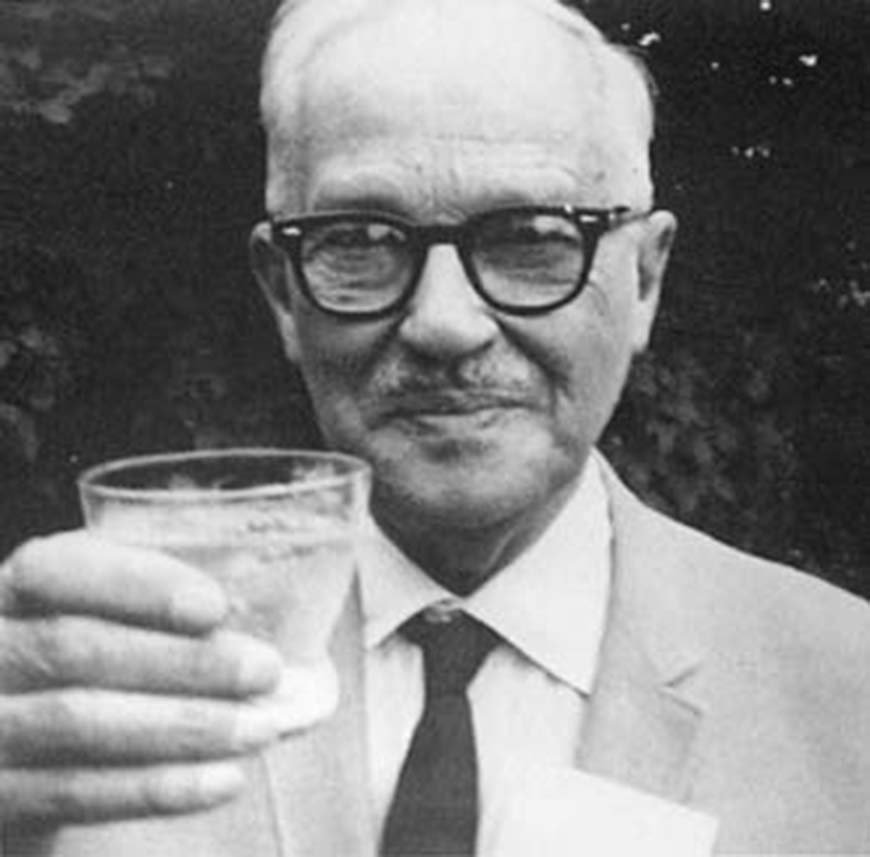
\includegraphics[width=0.9\columnwidth]{neyman.jpeg}
		\end{column}
	\end{columns}
\end{frame}

\begin{frame}{What are Confidence Intervals?}
	\begin{example}[Confidence Intervals of a Public Policy Analysis]
		Say you performed a statistical analysis to compare
		the efficacy of a public policy between two groups and you obtain a
		difference between the mean of these groups.
		You can express this difference as a confidence interval.
		Often we choose 95\% confidence.
		This means that \textbf{95 studies out of 100},
		that uses the \textbf{same sample size and target population},
		performing the \textbf{same statistical test},
		will expect to find a result of the mean difference between groups
		inside the confidence interval.
	\end{example}
	\footnotesize \textcolor{red}{Doesn't say anything about you \textbf{target population},
		but about you \textbf{sample} in an insane process of \textbf{infinite sampling} ...}
\end{frame}

\begin{frame}{Confidence Intervals versus Posterior Intervals}
	\centering
	\begin{tikzpicture}
		\begin{axis}[every axis plot, line width=2pt,
				xmin=0, xmax=4,
				ymin=0, ymax=1.5,
				ylabel=\empty,
				xlabel={$\theta$},
				samples=200,
				axis x line*=bottom, % no box around the plot, only x and y axis
				axis y line*=left,
				enlarge x limits=true, % extend the axes a bit
			]

			\addplot [blue, domain=0:4, forget plot] {lognormal(0, 2)};
			\addplot+ [
				mark=none,
				area legend,
				line width=0pt,
				color=blue,
				fill=blue, fill opacity=0.5,
				domain=0.25950495026507125:3.8534910373715427
			]
			{lognormal(0, 2)} \closedcycle;
			\addlegendentry{50\% Posterior}
			\addplot[red, mark=none] (-0.09, 1.4739034450607542) to (0.09, 1.4739034450607542);
			\addlegendentry{MLE}
			\draw [red] (0,0) to (0, 1.4739034450607542);
		\end{axis}
	\end{tikzpicture}
\end{frame}

\begin{frame}{Confidence Intervals versus Posterior Intervals}
	\centering
	\begin{tikzpicture}
		\begin{axis}[every axis plot, line width=2pt,
				xmin=-3, xmax=14,
				%ymin=0, ymax=1.5,
				ylabel=\empty,
				xlabel={$\theta$},
				samples=200,
				axis x line*=bottom, % no box around the plot, only x and y axis
				axis y line*=left,
				enlarge x limits=true, % extend the axes a bit
				%legend pos=outer north east, % there is one default value for the `legend pos' that is outside the axis
				%legend cell align=left, % so the legend looks a bit better
			]

			\addplot [blue, domain=-3:14, forget plot] {sumtwonormals(2, 1, 0.6, 10, 1, 0.4)};
			\addplot+ [
				mark=none,
				area legend,
				line width=0pt,
				color=blue,
				fill=blue, fill opacity=0.5,
				domain=1.8:9.7
			]
			{sumtwonormals(2, 1, 0.6, 10, 1, 0.4)} \closedcycle;
			\addlegendentry{50\% Posterior}
			\addplot[red, mark=none] (1.5, 0.24) to (2.5, 0.24);
			\addlegendentry{MLE}
			\draw [red] (2,0) to (2, 0.24);
		\end{axis}
	\end{tikzpicture}
\end{frame}

\begin{frame}{But why I never see stats without $p$-values?}
	\begin{columns}
		\begin{column}{0.8\textwidth}
			We cannot understand $p$-values if we do no not comprehend
			its origins and historical trajectory.
			The first mention of $p$-values was made by the statistician
			Ronald Fischer in 1925 \parencite{fisher1925statistical}:
			\begin{quotation}
				[$p$-valor is a] measure of evidence against the null hypothesis
			\end{quotation}
			\begin{vfilleditems}
				\item To quantify the strength of the evidence against the null hypothesis,
				Fisher defended ``$p<0.05$ as the standard level to conclude that there is evidence against the tested hypothesis''
				\item ``We should not be off-track if we draw a conventional line at 0.05''
			\end{vfilleditems}
		\end{column}
		\begin{column}{0.2\textwidth}
			\centering
			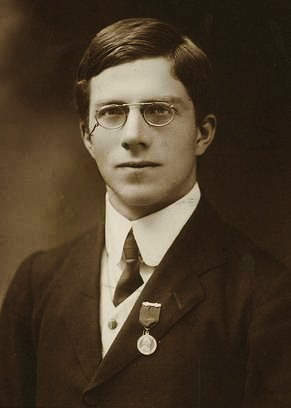
\includegraphics[width=0.9\columnwidth]{fisher.jpg}
		\end{column}
	\end{columns}
\end{frame}

\begin{frame}{$p = 0.06$}
	\begin{vfilleditems}
		\item Since $p$-value is a probability, it is also a continuous measure.
		\item There is no reason for us to differentiate $p = 0.049$ against $p = 0.051$.
		\item Robert Rosenthal, a psychologist said ``surely, God loves the $.06$ nearly as much as the $.05$''~\parencite{rosnow1989statistical}.
	\end{vfilleditems}
\end{frame}

\begin{frame}{But why I never heard about Bayesian statistics?\footnote{\textit{inverse probability}
			was how Bayes' theorem was called in the beginning of the 20th century}}
	\begin{columns}
		\begin{column}{0.8\textwidth}
			\begin{quotation}
				… it will be sufficient … to reaffirm my personal conviction …
				that the theory of inverse probability is founded upon an error,
				and must be wholly rejected.
			\end{quotation}
			\vfill \vfill
			\textcite{fisher1925statistical}
		\end{column}
		\begin{column}{0.2\textwidth}
			\centering
			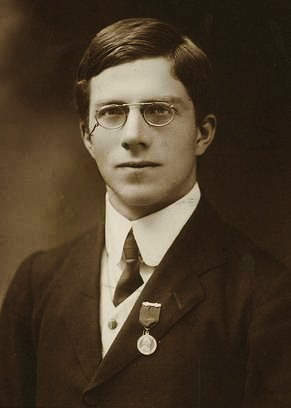
\includegraphics[width=0.9\columnwidth]{fisher.jpg}
		\end{column}
	\end{columns}
\end{frame}

\begin{frame}{Inside every nonBayesian, there is a Bayesian struggling to get out\footnote{
			quote from Dennis Lindley}}
	\begin{columns}
		\begin{column}{0.8\textwidth}
			\begin{vfilleditems}
				\item In his final year of life,
				Fisher published a paper \parencite{fisherExamplesBayesMethod1962}
				examining the possibilities of Bayesian methods,
				but with the prior probabilities being determined experimentally.
				\item Some authors speculate \parencite{jaynesProbabilityTheoryLogic2003}
				that if Fisher were alive today, he would probably be a Bayesian.
			\end{vfilleditems}
		\end{column}
		\begin{column}{0.2\textwidth}
			\centering
			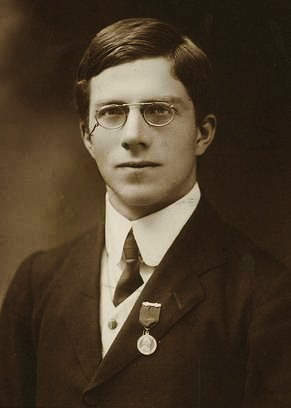
\includegraphics[width=0.9\columnwidth]{fisher.jpg}
		\end{column}
	\end{columns}
\end{frame}

\subsection{Bayesian Statistics}
\begin{frame}{Bayes' Theorem as an Inference Engine}
	\footnotesize Now that you know what is probability and Bayes' theorem,
	I will propose the following:
	$$
		\underbrace{P(\theta \mid y)}_{\text{Posterior}} = \frac{\overbrace{P(y \mid  \theta)}^{\text{Likelihood}} \cdot \overbrace{P(\theta)}^{\text{Prior}}}{\underbrace{P(y)}_{\text{Normalizing Constant}}}
	$$
	\begin{vfilleditems}
		\item \footnotesize $\theta$ -- parameter(s) of interest
		\item \footnotesize $y$ -- observed data
		\item \footnotesize \textbf{Priori}: prior probability of the parameter(s) value(s)
		\item \footnotesize \textbf{Likelihood}: probability of the observed data given the parameter(s) value(s)
		\item \footnotesize \textbf{Posterior}: posterior probability of the parameter(s) value(s) after we observed data $y$
		\item \footnotesize \textbf{Normalizing Constant}\footnote{sometimes also called \textit{evidence}.}: $P(y)$ does not make any intuitive sense.
		This probability is transformed and can be interpreted as something that only exists so that the result $P(y \mid \theta) P(\theta)$ be constrained between $0$ e $1$
		-- a valid probability.
	\end{vfilleditems}
\end{frame}

\begin{frame}{Bayes' Theorem as an Inference Engine}
	Bayesian statistics allows us to \textbf{quantify directly the uncertainty}
	related to the value of one or more parameters of our modelo given the
	observed data.
	This is the \textbf{main feature} of Bayesian statistics,
	since we are estimating directly $P(\theta \mid y)$ using Bayes' theorem.
	The resulting estimate is totally intuitive:
	simply quantifies the uncertainty that we have about the value of one or more
	parameters given the data, model assumptions (likelihood) and the prior
	probability of these parameter's values.
\end{frame}

\subsubsection{Advantages of Bayesian Statistics}
\begin{frame}{Bayesian vs Frequentist Stats}
	%\begin{table}[h!]
	\small
	\begin{tabular}{|l|p{.3\textwidth}|p{.3\textwidth}|}
		\toprule
		                     & \textcolor{blue}{\textbf{Bayesian Statistics}} & \textcolor{red}{\textbf{Frequentist Statistics}}                   \\ \midrule
		\textbf{Data}        & Fixed –- Non-random                            & Uncertain –- Random                                                \\ \midrule
		\textbf{Parameters}  & Uncertain –- Random                            & Fixed –- Non-random                                                \\ \midrule
		\textbf{Inference}   & Uncertainty regarding the parameter value      & Uncertainty regarding the sampling process from an infinite sample \\ \midrule
		\textbf{Probability} & Subjective                                     & Objective (but with several model assumptions)                     \\ \midrule
		\textbf{Uncertainty} & Posterior Interval –- $P(\theta \mid y)$       & Confidence Interval –- $P(y \mid \theta)$                          \\
		\bottomrule
	\end{tabular}
	%\end{table}
\end{frame}

\begin{frame}{Advantages of Bayesian Statistics}
	\begin{vfilleditems}
		\item Natural approach to express uncertainty
		\item Ability to incorporate previous information
		\item Higher model flexibility
		\item Full posterior distribution of the parameters
		\item Natural propagation of uncertainty
	\end{vfilleditems}
	\small \textbf{Main disadvantage}: Slow model fitting procedure
\end{frame}

\begin{frame}{The beginning of the end of Frequentist Statistics}
	\begin{vfilleditems}
		\small
		\item Know that you are in a very special moment in history of great changes in statistics
		\item I believe that frequentist statistics, specially the way we qualify evidence and hypotheses with
		$p$-values will transform in a ``significant''\footnote{pun intended ...} way.
		\item 6 years ago, the \textit{American Statistical Association} (ASA) published a declaration about
		$p$-values \parencite{Wasserstein2016}.
		It states exactly what we exposed here:
		The main concepts of the null hypothesis significant testing and,
		in particular $p$-values, cannot provide what researchers demand of them.
		Despite what says several textbooks, learning materials and published content,
		$p$-values below $0.05$ doesn't ``prove'' anything.
		Not, on the other way around, $p$-values higher than acima $0.05$ refute anything.
		\item ASA statement has more than 4.700 citations with relevant impact.
	\end{vfilleditems}
\end{frame}

\begin{frame}{The beginning of the end of Frequentist Statistics}
	\begin{vfilleditems}
		\small
		\item An international symposium was promoted in 2017 which originated an open-access special edition of
		\textit{The American Statistician} dedicated to practical ways to abandon $p < 0.05$
		\parencite{wassersteinMovingWorld052019}.
		\item Soon there were more attempts and claims.
		In September 2017, \textit{Nature Human Behaviour} published an editorial proposing that the $p$-value's
		significance level be decreased from $0.05$ to $0.005$ \parencite{benjaminRedefineStatisticalSignificance2018}.
		Several authors, including highly important and influential statisticians argued that this simple step would
		help to tackle the replication crisis problem in science, that many believe be the main consequence
		of the abusive use of $p$-values \parencite{Ioannidis2019}.
		\item Furthermore, many went a step ahead and suggested that science banish once for all $p$-values
		\parencite{ItTimeTalk2019,lakensJustifyYourAlpha2018}.
		Many suggest (including myself) that the main tool of statistical inference
		be Bayesian statistics \parencite{amrheinScientistsRiseStatistical2019, Goodman1180, vandeschootBayesianStatisticsModelling2021}.
	\end{vfilleditems}
\end{frame}
